\documentclass{article}

\usepackage[utf8]{inputenc} % set input encoding (not needed with XeLaTeX)

\usepackage{geometry}
\geometry{margin=2.5cm}

\usepackage{forest}
\usepackage{mathtools}

\usepackage{titlesec}
\titlespacing{\subsection}{0pt}{*6}{*1.5}
\renewcommand{\thesubsection}{SWT-\ifnum\value{subsection}<10\relax0\fi\arabic{subsection}}

\usepackage{tikz}
\usepackage{german}

\begin{document}
\title{\Large Einsendeaufgabe 1}
\author{\normalsize Stefan Berger}
\date{}
\maketitle

\subsection{Softwaretechnik allgemein}
\paragraph{}
Was ist Softwaretechnik? Was wird da gelehrt? Worum geht es?

\paragraph{}
Softwaretechnik ist ein systematischer, messbarer Ansatz zu Entwicklung, Betrieb und Wartung von
Software. Dabei geht es um Methoden, Werkzeuge, Maßsysteme, Standards und
Erfahrungen.

\subsection{Softwarelebenszyklus}
\paragraph{}
Sie werden in einem Bewerbungsgespräch gebeten, die wesentlichen Teile des Softwarelebenszyklus an dem Whiteboard zu skizzieren und zu erläutern. Können Sie das?

\paragraph{}
Eine Möglichkeit ist, den Softwarelebenszyklus in sechs Phasen zu unterscheiden.
Am Ende jeder Phase steht dann ein Phasenergebnis:

\paragraph{}
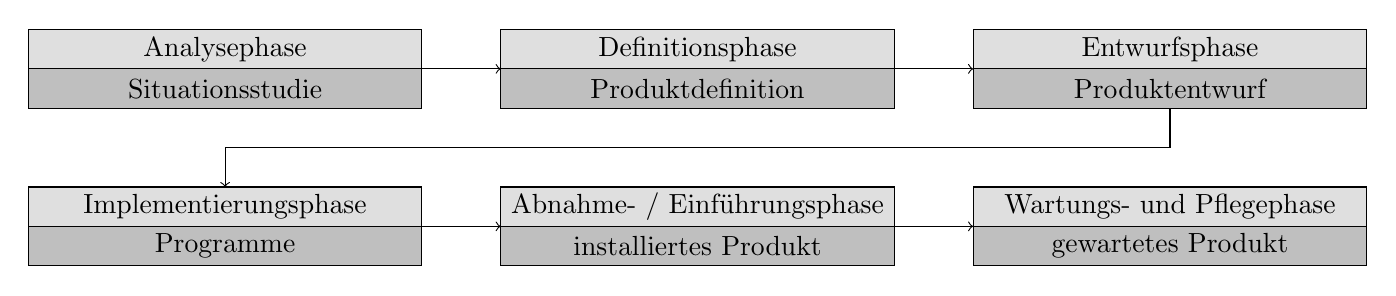
\begin{tikzpicture}
\draw [fill=gray!25](0,2.5) rectangle (5,3) node[pos=.5] {Analysephase};
\draw [fill=gray!50](0,2) rectangle (5,2.5) node[pos=.5] {Situationsstudie};

\draw[->] (5,2.5) -- (6,2.5);

\draw [fill=gray!25](6,2.5) rectangle (11,3) node[pos=.5] {Definitionsphase};
\draw [fill=gray!50](6,2) rectangle (11,2.5) node[pos=.5] {Produktdefinition};

\draw[->] (11,2.5) -- (12,2.5);

\draw [fill=gray!25](12,2.5) rectangle (17,3) node[pos=.5] {Entwurfsphase};
\draw [fill=gray!50](12,2) rectangle (17,2.5) node[pos=.5] {Produktentwurf};

\draw (14.5,2) -- (14.5,1.5);
\draw (14.5,1.5) -- (2.5,1.5);
\draw[->] (2.5,1.5) -- (2.5,1);

\draw [fill=gray!25](0,.5) rectangle (5,1) node[pos=.5] {Implementierungsphase};
\draw [fill=gray!50](0,0) rectangle (5,.5) node[pos=.5] {Programme};

\draw[->] (5,.5) -- (6,.5);

\draw [fill=gray!25](6,1) rectangle (11,.5) node[pos=.5] {Abnahme- / Einführungsphase};
\draw [fill=gray!50](6,0) rectangle (11,.5) node[pos=.5] {installiertes Produkt};

\draw[->] (11,.5) -- (12,.5);

\draw [fill=gray!25](12,1) rectangle (17,.5) node[pos=.5] {Wartungs- und Pflegephase};
\draw [fill=gray!50](12,0) rectangle (17,.5) node[pos=.5] {gewartetes Produkt};
\end{tikzpicture}

\subsection{Prinzipien}
\paragraph{}
Geben Sie bitte zu jedem Prinzip der Softwaretechnik (Abstraktion, Strukturierung, Hierarchisierung, Modularisierung, Standardisierung) ein Beispiel an. Wo ist Ihnen das schon begegnet und wo könnte das in der Softwaretechnik angewendet oder wirksam werden?

\paragraph{}
Abstraktion: Abstrakte Klassen sind ein typisches Beispiel. Von ihnen müssen
erst konkrete Unterklassen gebildet werden, bevor Objekte erstellt werden
können. Beispiele sind die Klassen "`Person"', "`Fahrzeug"' und "`Lebewesen"'.

\paragraph{}
Strukturierung: UML-Strukturdiagramme bieten die Möglichkeit, die Entwicklung
einer Software oder die Software selbst zu strukturieren. Durch sie wird das
Zusammenwirken z.B. von Komponenten oder Paketen verdeutlicht.

\paragraph{}
Hierarchisierung: Das beste Beispiel für eine Hierarchie im Softwarebereich sind
Verzeichnisbäume. In der objektorientierten Programmierung gibt es
Klassenhierarchien. Die Aufbauorganisation im Betrieb ist ein weiteres Besipiel
für eine Hierarchie aus dem organisatorischen Bereich.

\paragraph{}
Modularisierung: Module gibt es in der Software z.B. in Form von Plugins. Die
IDE Eclipse ist zusammengesetzt aus vielen Modulen für die Entwicklung in
verschiedenen Programmiersprachen und von verschiedenen Softwarearten.

\paragraph{}
Standardisierung: ASCII und UTF-8 gehören zu den berühmtesten Standards im
Softwarebereich. UML, XML und die Programmiersprache Java sind standardisierte
Sprachen.

\subsection{Recherche}
\paragraph{}
Recherchieren Sie bitte im Internet über Softwaretechnik oder Softwareengineering. Welche Bereiche interessieren Sie ganz besonders?

\paragraph{}
Mich interessiert das gesamte Spektrum der Softwaretechnik. Als
Anwendungsentwickler habe ich Erfahrungen mit der Implementierung und dem
Testen von Software. Die nächsten Recherchen werden sich mit den diesen vor-
und nachgelagerten Phasen beschäftigen. Entwickler benötigen eine durchdachte
Konzeption und ein effizientes Design der Software, um die Software korrekt
implementieren zu können. Nach der Umsetzung müssen das Projekt übergeben und
die Benutzer geschult werden.

\subsection{Wissensfragen zur Lerneinheit}
\paragraph{}
Versuchen Sie die Fragen schriftlich zu beantworten ohne noch einmal in der Lerneinheit nachzuschlagen.

\paragraph{1}
An welche Best Practices erinnern Sie sich oder welche haben Sie verinnerlicht? \\

Best Practices sind z.B. Prozessmodelle wie Wasserfall, Scrum, etc. Das
Verwenden von IDEs und das Berücksichtigen von Standards gehören auch zu den
Best Practices.

\paragraph{2}
Warum ist es sinnvoll Softwarefehler früh zu erkennen?

\paragraph{}
Je später ein Softwarefehler erkannt und behoben wird, desto höher sind die
Kosten dafür.

\paragraph{3}
Was geht in Softwareprojekten typischerweise schief?

\paragraph{}
Die häufigsten Fehler treten in der Systemlogik auf, gefolgt von Dokumentationsfehlern,
Abarbeitungsfehlern im Rechner und Fehlern im Code. Seltener sind Datenbehandlungsfehler,
Fehler in den Anforderungen, im Prozessverlauf oder der Hardware die Ursache.

\paragraph{4}
Kennen Sie (Standardisierungs-)Organisationen, die sich mit Software beschäftigen?

\paragraph{}
IEEE, DIN, ISO, ANSI, DoD, ACM, DEN, GI

\subsection{Fehlerquellen}
s. SWT-05 Antwort 3

\subsection{Phaseneinteilung}
s. SWT-02













\end{document}
